\chapter{Implémentation et évaluation du système}\label{eval}

Au chapitre précédent, nous avions extraits des informations précieuses de VerbNet. Dans ce chapitre, nous expliquerons comment nous nous sommes servis des informations extraites en Python. Nous avons d'abord implémenter les dictionnaires dans GenDR. Puis nous nous sommes servis des structures générées pour plus rapidement construire les graphes sémantiques. Ceux-ci nous serviront à tester notre système. Cette section est séparée en trois parties. D'abord nous expliquons comment les dictionnaires sont architecturés mainantent. Puis nous expliquerons en quoi certaines règles de grammaire ont changé à l'aide d'un exemple retraçant la construction d'un arbre. Puis finalement, nous parlerons de l'évaluation en soi.

\section{Implémentation des verbes et de leurs patrons de régime: lexicon.dict et gpcon.dict}

Au chapitre \ref{chapgendr}, nous avons démontré comment l'information lexicale était encodée dans GenDR. Nous avions deux dictionnaires: semanticon et lexicon. Ici, nous en avons trois: semanticon, lexicon et gpcon. L'implémentation de VerbNet a donc eu pour effet la création d'un troisième dictionnaire et la modification du lexicon. Effectivement, l'architecture du semanticon est restée la même.

\subsection{Lexicon.dict 2.0}
Commençons par le lexicon. Anciennement le lexicon de GenDR était structuré ainsi: une diathèse triviale est encodée dans predicate, puis les classes verbales sont de trois types: verbes à 1 actant (sujet), verbe à un actant (transitif direct), verbe à un actant transitif indirect, verbe à deux actants ditransitif. Puis, en ce qui concerne les verbes, chaque verbe doit pointer vers un des types de verbes. Puis à l'intérieur du verbe, si un des actants syntaxiques a des contraintes particulières on l'encode là. Voir la figure \ref{lexicon}.

Dorénavant, le lexicon fonctionne ainsi:
attributs par défaut de toutes les classes: 
Verbes
Noms
Adjectifs
etc.

Voici à quoi les noms et verbes ressemblent.
\begin{lstlisting}[language=XML, caption = Attributs par défaut des classes]
// ================= VERBS =================

// VERB
// ----

verb {
  dpos = V
  spos = verb
}

// ================= NOUNS =================

// NOUN
// ----
// Common nouns.

noun {
  dpos = N
  spos = noun
  countable = yes
  gp = { id=NP dia=1}
}
\end{lstlisting}

Ensuite on liste tous les verbes (6393) qui pointent vers une classe verbale (de tout niveau de profondeur). Il s'agit de la partie qu'on a extrait à la figure \ref{extracmembre}.
Ça ressemble à cela

\begin{lstlisting}[language=XML, caption = Partie membre du lexicon]
/*
 =======================================================
                      VERBNET MEMBERS
 =======================================================
*/
open_5 : "spatial_configuration-47.6"
open_up : "establish-55.5-1"
operate : "other_cos-45.4"
oppose : "amalgamate-22.2-3"
ordain : "appoint-29.1"
order_1 : "get-13.5.1"
order_2 : "order-60-1"
organize_1 : "create-26.4"
organize_2 : "establish-55.5-1"
organize_3 : "force-59-1"
originate : "establish-55.5-1"
ornament_1 : "butter-9.9"
ornament_2 : "fill-9.8"
ornament_3 : "illustrate-25.3"
\end{lstlisting}

Montrer qu'on a pu le système des classes predicate, verb dt, verb dit, etc. Que maintenant on a juste verb pour la dpos et la spos. Le reste est encodé directement dans chaque classe verbale de VerbNet : diathèse, id des patrons (pas de fonctions lex.). Montrer comment les mécanismes d'héritage fonctionnent maintenant : members vers classe verbale et classe verbale vers 'verb' ou vers leurs classes mères pour hériter de leurs gps, etc. Montrer un exemple d'une lexie (parler de la désambiguisation) qui pointe vers une sous-classe donc qui hérite des trais de la classe et de leurs gps, etc. Expliquer comment nous avons contruit cette partie et comment ça fonctionne. ON réitère la diathèse à chaque gp, pas comme dans l'autre lexicon où une diathèse triviale est donnée à tous, et quand elle change, on l'explicite ponctuellement dans une entrée donnéequi en aurait besoin.

\begin{lstlisting}[language=XML, caption = Partie: Classes de VerbNet]
/*
=======================================================
                   VERBNET CLASSES
=======================================================
*/

"tell-37.2": verb {
  gp = { id=NP_V_NP  
	       dia=12 } // John informed me.
  gp = { id=NP_V_NP_PP_of_topic  
	       dia=123 } // John informed me of the situation. }
"tell-37.2-1": "tell-37.2" {
  gp = { id=NP_V_NP  
	       dia=12 } // Ellen told a story.
  gp = { id=NP_V_NP_PP_to_recipient 
		     dia=123 } // Ellen told a story to Helen.
  gp = { id=NP_V_NP_Dative_NP   
	       dia=132 } // Ellen told Helen a story. Ellen told me, 'Leave the room.'
  gp = { id=NP_V_NP
		     dia=13 } // Ellen told Helen.
  gp = { id=NP_V_NP_PP_about_topic
		     dia=132 } // Ellen told Helen about the situation.
}
\end{lstlisting}

Ensuite nous avons le reste du lexique: noms, adjectifs, adverbes, prépositions, déterminants,etc. Les entrées sont normalement vides, sauf lorsqu'elles font appel à une fonction lexicale. Nous n'avons encodé que l'usage des fonctions lexicales locatives de type: Locin, Locad, Locab. Elles fonctionnent lorsqu'une unité lexicale sélectionne la préposition à utiliser et non le verbe. C'est pourquoi elles sont encodées sous le nom qui la sélectionne. (j'en aurai parlé à la section précédente)

\begin{lstlisting}[language=XML, caption = Partie: Unités lexicales non-verbales]
/*
=======================================================
               NON-VERBAL LEXICAL ENTRIES     
=======================================================
*/
accountant : noun
acorn : noun
acquaitance  : noun
across : preposition
\end{lstlisting}

Maintenant que nous avons fini d'expliquer le nouveau lexicon. Passons au dictionnaire qui contient tous les propriétés syntaxiques des ID que nous avons vu à la figure X.

\subsection{gpcon.dict}
Le gpcon, un dictionnaire de patron de régime qui contient 278 identifiants de patrons de régime.
expliquer comment le lexicon fait appel au gpcon et pourquoi on l'a encodé ainsi. le id dans gp d'une entrée pointe vers une entrée de gp dans le gpcon. Celui-ci contient toutes les informations du patron de régime. Le fait de séparer les dictionnaires comme ça ressemble bcp aux méthodes vues par XTAG, FrameNet, FORGe,  etc. Les unités dans le gpcon sont les identifiants des GPS. Puis à l'intérieur on spécifie les propriétés syntaxiques. On spécifie le nombre d'actant syntaxique en jeu. L'union de ça et de la diathèse dans l'autre dictionnaire permet de rendre compte des phénomènes où 2 gps utilisent les mêmes actants, mais qu'en surface on les réalise dans des ordres différents avec des prépositions différentes ou sans prépositions. Donc l'ordre des actants syntaxiques est important puisque la diathèse se base là dessus. Puis les informations syntaxiques dans les actants sont utiles pour que le premier actant est contraint d'être un N par exemple, puis son deuxième un V. Puis de l'information de surface: la relation. Cela dicte au système comment appelé la relation entre le dépendant et son gouverneur. Cela fait en sorte que si on prend le premier GP \lstinline! NP_agent_V { I={rel=subjective dpos=N} }!, quand on utilise le patron de régime identifié comme Np agent V on veut que son premier actant syntaxique soit de type nominal et que sa réalisation de surface est une relation subjective. Nous avons aussi instauré un mécanisme pour tenir compte du fait que certains patrons de régime permettent deux prépositions qui compétitionnent pour le même actant syntaxique. c'est le cas quand on regarde le gp \lstinline!NP_asset_V_NP_PP_from_out_of! qui a dans son régime \lstinline!III={rel=oblique dpos=N prep=from}! et \lstinline!III={rel=oblique dpos=N prep="out of"}!. Ainsi, cela permet de paraphraser encore plus et nous pouvons tenir compte du fait que VerbNet avait spécifié cela. Finalement, en créant notre dictionnaire de patron de régime, nous nous sommes rendus compte qu'il existait énormément de doublons. Nous en avons un exemple dans cet extrait de dictionnaire. Np agent V et NP attribute V ont les mêmes propriété syntaxiques. Ce sont deux identifiants qui représentent la même chose. Ce scénario se répète souvent dans notre gpcon. C'est une conséquence de VerbNet qui considère qu'il s'agit de deux gps différents puisque les rôles thématiques sont utilisés dans VerbNet. Comme nous les remplaçons par des actants sémantiques puis syntaxiques, que ce soit un agent ou un attribut ne change pas grand chose. Comme nous voulions tester l'implémentation de VerbNet, nous n'avons pas pris le temps de remédier à cette situation, mais elle n'était pas encombrante. On pourrait prendre le temps de nettoyer le dictionnaire de patron de régime.

\begin{lstlisting}[language=XML, caption = Gpcon]
NP_agent_V {
   I={rel=subjective dpos=N}
}
NP_agent_V_NP {
   I={rel=subjective dpos=N}
   II={rel=dir_objective dpos=N}
}
NP_asset_V_NP_PP_from_out_of {
   I={rel=subjective dpos=N}
   II={rel=dir_objective dpos=N}
   III={rel=oblique dpos=N prep=from}
   III={rel=oblique dpos=N prep="out of"}
}
NP_attribute_V {
   I={rel=subjective dpos=N}
}
\end{lstlisting}

\section{Ajustement du module grammatical: un exemple}
Maitenant que nous avons montré à quoi les dictionnaires ressemblent, nous allons présenter un exemple servant à exemplifier comme les règles de grammaires et les dictionnaires interagissent. Cela nous permettra aussi de présenter les nouvelles règles et mécansimes utilisés pour l'implémentation de VerbNet.

\subsection{Input}
La phrase: The teacher talked about history to the students. Décrire un peu l'input

\begin{lstlisting}[language=XML, caption=Input textuel, label=text-input]
structure Sem S {
  S:1{
    talk_3:1{
      tense=PAST 
      1-> teacher:1
      2-> student:1
			3-> history:1
    }
    teacher:1{number=SG definiteness=DEF}
    history:1{number=SG definiteness=NO}
    student:1{number=PL definiteness=DEF}
    main-> talk_3:1
  }
}
\end{lstlisting}

L'input de la figure \ref{text-input} permet de générer 9 arbres de syntaxe profonde qui correspondent aux phrases suivantes : 1)The teacher talked, 2)The teacher talked to the students, 3)The teacher talked with the students, 4)the teacher talked to the students about history, 5)The teacher talked with the students about history, 6)the teacher talked, 7)the teacher talked about history to the students, 8)the teacher talked about history with the students, 9)the teacher talked about history.

Ces 9 arbres découlent des patrons de régime permis par le lexème \lex{talk\_3} qui pointe vers la classe "talk-37.5". Donc 9 structures profondes ont été réalisées à partir de cet input parce que tous les gp permettaient de prendre le graphe sémantique en entrée. L'input contenait 3 arguments: les actants sémantiques 1,2 et 3. Et tous les patrons de régime ici sont des combinaisons de ces 3 actants. D'ailleurs pour qu'un patron s'applique, il peut y avoir plus d'actants dans la structure sémantique, ça ne posera pas problème, car la manière qu'il choisi de réaliser le gp dépend de s'il est applicable ou non (expliquer avec gp selection). La raison pour laquelle les 9 gps ont été réalisés sera plus claire lorsque nous aurons passé au travers de l'exemple. Pour l'instant, nous allons prendre la strcuture syntaxique profonde qui aurait généré la phrase que nous souhaitons reproduire. Soit la 4e structure

\begin{lstlisting}[language=XML, caption=Input textuel de l'exemple]

"talk-37.5": verb {
  gp = { id=NP_V                           dia=1 } // Susan talked.
  gp = { id=NP_V_PP_to_co_agent            dia=12 } // Susan talked to Rachel.
  gp = { id=NP_V_PP_with_co_agent          dia=12 } // Susan talked with Rachel.
  gp = { id=NP_V_PP_to_co_agent_PP_about_topic dia=123 } // Susan talked to Rachel about the problem.
  gp = { id=NP_V_PP_with_co_agent_PP_about_topic dia=123 } // Susan talked with Rachel about the problem.
  gp = { id=NP_V                           dia=12 } // Susan and Rachel talked.
  gp = { id=NP_V_PP_about_topic_PP_to_co_agent dia=132 } // Susan talked about the problem to Rachel.
  gp = { id=NP_V_PP_about_topic_PP_with_co_agent dia=132 } // Susan talked about the problem with Rachel.
  gp = { id=NP_V_PP_about_topic            dia=13 } // Susan talked about the problems of modern America.
}
\end{lstlisting}

\subsection{Création et lexicalisation de la racine}:
D'abord, la première règle appliquée est la règle de racine (root\_standard). Elle crée la racine de l'arbre et impose une dpos=V et une finitude=FIN. Puis le noeud dominant en RSem est lexicalisé s'il satisfait les contraintes requises. La lexicalisation de talk\_3 est opérée grâce à la règle lex\_guess\_from\_lexicon. Nous en avions glissé un mot au chapitre \ref{chapgendr} lorsque nous parlions des règles de lexicalisation fallback qui permettent de déduire que le lexème talk\_3 qu'on retrouve dans le dictionnaire est probablement la correspondance du sens de \sem{talk\_3} qu'on aurait retrouvé dans le dictionnaire. D'ailleurs, c'est logique puisque talk\_2 et talk\_1 n'ont pas le même sens, donc on les sépare. Jusqu'à présent les deux premières règles sont identiques à GenDR comme nous l'avons vu à la section \ref{secexemple}.

\begin{figure}[htb]
	\centering
	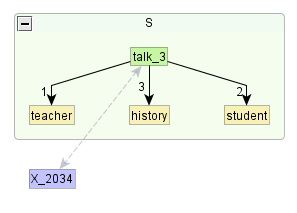
\includegraphics[width=0.5\textwidth, trim = {0cm 0cm 0cm 0cm},clip]{ch6/figs/root.png}
	\caption{Création de la racine à partir du noeud dominant}
	\label{deroulement0}
\end{figure}


\subsection{Sélection du patron de régime dans le lexicon}:
Ensuite, une fois que le noeud dominant est lexicalisé, la règle actant\_gp\_selection embarque. Ce qu'elle fait: elle prend le noeud (talk 3) puis elle regarde si cette entrée a un trait gp. Si oui, elle regarde dans le trait gp à la recherche de traits dia et id. ID est l'identifiant d'un patron de régime et dia fait en sorte que le gp sélectionnée se fasse en fonction de la disponibilité des actants sémantiques. Le trait dia nous dit aussi dans quel ordre les actants sémantiques se retrouvent en syntaxe.Il est essentiel qu'un lexème verbal aille chercher ces traits car il en a besoin pour appliquer les règles actancielles qui en découlent. Il faut que le système sache quel patron de régime utilisé pour un prédicat donné, et dans quel ordre les actants seront réalisés en syntaxe. La règle impose un gp au lexème en fonction de la diathèse du gp (quels actants sémantiques sont nécessaires à l'application du gp). Donc, de cette manière on s'assure que, après que la racine soit lexicalisée, seulement un gp traitant les actants sémantiques demandés en input sera utilisé. Dans le cas inverse, l'arborisation s'arrête brusquement après. Si la classe verbale contenait un gp dont la dia était 1234 ou bien 14, alors la réalisation n'aurait pas fonctionné, car il n'y a pas de quatrième actant dans la structure sémantique.

\begin{figure}[htb]
	\centering
	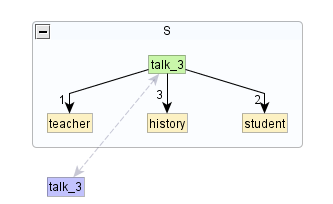
\includegraphics[width=1\textwidth, trim = {0cm 0cm 0cm 0cm},clip]{ch6/figs/selectiongp.png}
	\caption{Application de la règle actant\_gp\_selection}
	\label{deroulement1}
\end{figure}

\subsection{Règle actancielle: actant gp ijk}
Donc à l'étape précédente, le noeud lexical talk\_3 se fait imposer les restrictions suivantes: l'identification d'un gp et la diathèse qui vient avec. Cela va nous permettre d'appliquer cette règle. La règle actant gp ijk fait partie du groupe de règles actancielles que nous avons codés dans la grammaire. Dans GenDR, on regardait chaque arc individuellement, et on le faisait correspondre à une actant syntaxique dans le gp de l'entrée. Cela créait un arc entre la racine et un noeud vide mais contraints par les contraintes du gp. Maintenant ça ne fonctionne plus comme ça. Une fois que le gp est sélectionné, comme il a une diathèse de 3 actants sémantiques, il se fera imposer la règle qui réalise les relations actancielles à 3 actants (d'où le ijk). Nous en avons 6 pour réaliser des structures à 6 arguments. Dans notre cas, il fallait actant gp ijk.

La règle actant ijk, crée 3 arcs en partance talk\_3 au bout desquels se trouvent des noeuds vides sans contraintes. Les conditions pour que cette règle s'applique sont les suivantes: on veut que le noeud qui déclenche la règle soit lexicalisé, ait un patron de régime, et ait 3 actants sémantiques (les variables ijk). D'ailleurs, c'est à cette étape que le diathèse s'applique. Donc le passage des arcs sémantiques à syntaxique. Puisque la diathèse du gp X disait dia=123, cela se traduit par l'actant syntaxique I correspond au premier, puis ainsi de suite. Si on avait voulu que l'actant 2 soit l'actant syntaxique III, on aurait écrit la diathèse dia=132. Voir la figure \ref{deroulement2} \draft{en fait y'a un changement de diathèse, c'est pas la triviale, II devient 3 et III devient 2}

\begin{figure}[htb]
	\centering
	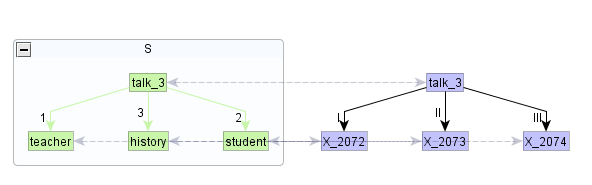
\includegraphics[width=1\textwidth, trim = {0cm 0cm 0cm 0cm},clip]{ch6/figs/actant_gp_ijk.png}
	\caption{Application d'une règle actancielle: actant\_gp\_ijk}
	\label{deroulement2}
\end{figure}

\subsection{Application des contraintes sur les noeuds}
Ensuite, il faut contraindre les noeuds créés lors de l'application de la règle précédente. Puisque avant les contraintes sur les noeuds se faisaient en utilisant le gp qui était dans le lexicon, on pouvait créer le noeud et le contraindre en même temps. Maintenant les restrictions sur les noeuds sont dans le gpcon, c'est pourquoi il faut une étape de plus. Donc cette règle dicte au système de regarder dans le gpcon pour le id du gp qui avait été sélectionné et contraindre les noeuds syntaxiques en fonctions des restrictions qu'ils ont (comme la dpos ou la finitude). La règle s'applique donc 3 fois puisqu'il y a trois noeuds vides. Voici les contraintes qu'on retrouve 

\subsection{lex standard}
Ensuite, on répète la règle de lexicalisation, puisque des noeuds vides n'attendent qu'à être lexicalisés s'il y a des lexèmes dans le lexicon qui peuvent satisfaire les contraintes des noeuds imposées à la règle précédente et qui correspondent à l'unité sémantique donnée en input. Dans cet exemple, c'est le cas et la règle lex\_standard s'applique donc 3 fois car il y a 3 noeuds à combler. Voir la figure \ref{deroulement3}

\begin{figure}[htb]
	\centering
	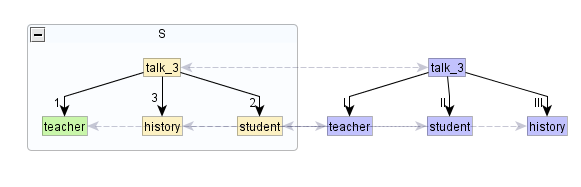
\includegraphics[width=1\textwidth, trim = {0cm 0cm 0cm 0cm},clip]{ch6/figs/lex.png}
	\caption{Application d'une règle de lexicalisation: lex\_standard}
	\label{deroulement3}
\end{figure}

\subsection{actant gp selection}

Finalement, la règle actant gp selection s'applique pour chaque noeud lexicalisé. Donc, à la fin, les lexèmes \lex{teacher},\lex{student} et \lex{history} ont leurs traits lexicaus en plus de l'identifiant d'un gp qui se trouve sous leur entrée et de la diathèse qui va de paire avec ce gp. Comme ce sont tous des noms communs, ils héritent du gp par défaut de la classe nominale. encore puisque ces nouveaux noeuds lexicalisés déclenchent l'application de la règle. Dès qu'un x a un gp, on va le repêcher, même si on s'en sert pas après. Dès qu'un noeud est lexicalisé, on regarde quel est son gp et on lui impose un gp. C'est pour cela qu'on se retrouve avec 9 réalisation profondes différentes. Parce que le verbe principal a 9 gps, sa lexicalisation a donc déclenché 9 occurrences de actant gp selection puisque le système scan pour tous les gps possibles et il créera un arbre différent à chaque fois.

Bref, grâce à toutes ces règles, nous avons opéré le passage de la RSem de x à la RSyntP de celle-ci. Une fois l'arborisation terminée, nous allons passé à structure syntaxique de surface.

\subsection{Lexicalisation des unités lexicales}
D'abord on applique une règle de lexicalisation de surface. Donc on va chercher deux traits: le lexicalisation de surface et la partie du disours de surface. Bref, c'est une simple règle de lexicalisation qui lexicalise les lexèmes à un niveau superficiel.

\subsection{Règles actancielles de surface}
Une fois que les lexèmes sont réalisés en surface, les règles actancielles de surface se réalise. 3 règles actancielles seront appliquées puisqu'il y a 3 arcs de dépendances à réaliser. Cela fait en sorte qu'au lieu d'avoir l'étiquette des chiffres romains pour exprimer la dépendance syntaxique, on utilise le nom des relations. Donc, la règle synt\_subj est déclenchée et la relation subjective est belle et bien encodée dans le patron de régime de l'actant syntaxique I du patron de régime sélectionné \emph{NP\_V\_PP\_to\_co\_agent\_PP\_about\_topic}: \lstinline! I={rel=subjective dpos=N}!. Puis la règle actancielle de surface synt\_actant\_prep est déclenchée une première fois pour la relation syntaxique II entre talk et history, ce qui nous donne \lstinline! II={rel=oblique dpos=N prep=about}! que l'actant syntaxique II est identifiée par la relation oblique entre le dépendant et son gouverneur, puis il y a une préposition. Donc le noeud où était history se scinde en 2 pour que la préposition qui était encodées dans les traits de l'actant syntaxique soit réalisée en syntaxe de surface. Il s'agit d'un mot fonctionnel. Comme vous pouvez le voir dans la figure \ref{deroulement4}. Puis la règle synt\_actant\_prep est appliquée une seconde fois pour réaliser la relation syntaxique entre student et talk en syntaxe de surface. Encore une fois le noeud est scindé en deux pour laisser place à la préposition \lex{to} qui sera l'intermédiaire entre le verbe et l'actant syntaxique. La relation générée est objet indirect.

\subsection{Règles des déterminants}
La règle det\_def réalise les déterminants qui doivent apparaître en syntaxe de surface. Ils correspondent aux traits que nous avions encodés dans l'input de départ. Seul \lex{teacher} et \lex{student} auront des déterminants puisque leur équivalent sémantique demandaient des définitudes qui s'était transmis jusqu'à la syntaxe profonde. Mais sont seulement réalisés en syntaxe de surface puisque ce sont des mots fonctionnels. La règle de déterminant réalise \lex{the} lorsque c'est défini et \lex{a} lorsque le noeud est marqué comme indéfini. C'est une règle propre à l'anglais.

\begin{figure}[htb]
	\centering
	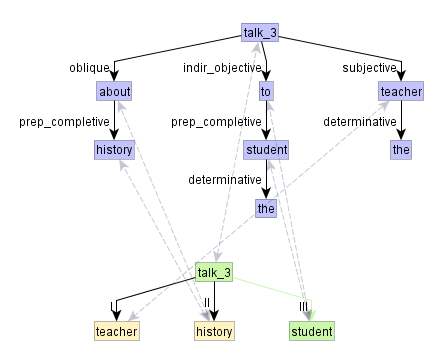
\includegraphics[width=1\textwidth, trim = {0cm 0cm 0cm 0cm},clip]{ch6/figs/ssynt.png}
	\caption{Applications des règles actancielles et réalisation des lexèmes fonctionnels}
	\label{deroulement4}
\end{figure}

Cela met fin à notre section implémentation. Nous avons démontré comment s'organisaient nos dictionnaires dorénavant et les nouvelles règles de grammaire qui ont tenu compte des changements apportés aux dictionnaires. Nous passerons donc à la phase évaluation pour voir comment a performé notre nouveau système.

\section{Évaluation}
Avant d'entrer dans le vif du sujet, il serait pertinent de faire un bref retour sur les méthodes classiques d'évaluation en \ac{GAT}. \cite{ReiterBuildingNaturalLanguage2000} soulignent déjà dans leur livre qu'une évaluation humaine de tels systèmes est la meilleure manière de procéder. Toutefois, environ une décennie plus tard, \cite{ReiterInvestigationValidityMetrics2009} remarquaient que les méthodes d'évaluation métriques se faisaient de plus en plus populaires. Notamment la méthode BLEU qui avait été développée pour les systèmes de traductions automatiques.'BLEU and related metrics work by comparing the output of an MT system to a set of reference translations (human translations of the source text), and in principle this kind of evaluation could be done with NLG systems as well.' 'As in other areas of NLP, the advantages of automatic corpus-based evaluation are that it is potentially much cheaper and quicker than human-based evaluation, and that it is repeatable. Indeed, NLG researchers have used BLEU in their evaluations for some time (Langkilde 2002; Habash 2004).'Nous avons donc considéré les diverses méthodes d'évaluation existant avant de prendre notre décision.

Toutefois, certains réalisateurs mettent en garde contre la méthode BLEU. D'ailleurs, lors de son passage à SemEval, FORGe a aussi été évalué à la fois avec BLEU, et avec des évaluations humaines. Toutefois, FORGe mettent en garde que BLEU est bon pour évaluer la couverture mais pas nécessairement la qualité de chaque output (p.922-923). Leur système avait un score au dessus de la moyenne pour ce qui était de l'évaluation humaine. Mais un score plus faible pour la méthode BLEU et ce en raison de la couverture car FORGe avait mis de l'avant la qualité de ses outputs de sorte que son système filtre à deux reprises dans le pipeline des constructions fautives ou potentiellement fautives.

Bref, La qualité des textes générés en GAT a été évaluée de diverses manières dans le passé. On pourrait tous les classés dans les catégories suivantes: task performance, human judgement and ratings et comparaison à des textes de corpus en utilisant des métriques automatiques \citep{ReiterInvestigationValidityMetrics2009}. Considérant ces choix classiques, nous devons exclure task performance et les méthodes métriques pour deux raisons. D'abord notre système ne réalise pas du texte dans un but précis. Donc on ne peut pas savoir si la phrase réalisée permet à un utilisateur d'accomplir une tâche en lisant le texte. Nous ne pouvons pas utiliser la méthode métrique car notre système génère des arbres de dépendances de surface. Les systèmes utilisant des métriques comparent les textes générés automatiquement avec des corpus de texte écrits par des humains. Pour comparer nos outputs, ils faudraient qu'ils soit morphologisé et linéarisé, ce qui n'est pas le cas. Nous n'avons donc qu'une méthode d'évaluation devant nous: l'évaluation humaine basée sur des jugements.

\subsection{Mise en place de l'évaluation}
D'abord, pour procéder à l'évaluation de notre système, nous avons pensé utiliser les phrases servant d'exemple que VerbNet a mis dans sa base de données. Nous nous sommes dit qu'il serait intéressant de prendre ces phrases, d'en extirper les unités sémantiques et construire des graphes sémantiques qui représentent ces énoncés. Au chapitre précédent, nous avons expliqué comment nous avons extrait ces phases exemples. Donc, la première étape était de prendre les 978 phrases et d'en faire 978 graphes sémantiques.

Après, nous avons pris 75 structures au hasard. De ceux-là nous avons pris 25 au hasard qui ont servi de développement pour voir les pépins immédiats. Dans la partie DEV nous avons remarqué que bon nombre de réalisations échouaient parce que l'input sémantique était deffectueux. Nous avons donc passé les 25 au peigne fin. Puis ensuite, un autre problème récurrent était que certains mots du lexique apparaissent en double dans notre dictionnaire. Par exemple le verbe \lex{work} et le nom \lex{work} s'écrivent de la même manière et le système construit l'arbre syntaxique à partir du premier qu'il voit. C'est pourquoi nous avons procédé à un filtrage massif de ces cas et nous l'avons réglé en mettant une entrée sémantique dans le semanticon qui contient deux entrées lexicale. Une version verbale et une version nominale (on les distingue en mettant un \_n pour les noms.) ex : semanticon : work : lex=work lex=work\_n. C'est pas systématique de mettre le n après chaque nom,c'est seuelemnt quand y'a conflit de deux entrées identiques. La désambiguisation fait en sorte que class\_1 et class\_2 existent donc, dans notre exemple, nous n'avions pas à mettre class\_n dans l'entrée. Cela mit fin à la partie DEV.  Nous n'avons pas analysé en profondeur la nature des générations de ce niveau, nous voulions seulement corriger les problèmes de surface. Ceux-ci étaient les plus marquants et populeux.

Nous sommes ensuite passé à la phase d'évaluation comme telle. Nous avons donc pris les 50 restants et nous les avons passé au système. Nous avons donc regardé chaque input de la partie EVAL pour nous assurer qu'ils soient en ordre, et nous avons scruté le lexique pour qu'il n'y ait pas de contradiction. et Nous avons finalement testé le système. Pour ce faire, nous avons développé un script permettant de visualiser les outputs de chaque input à tous les niveaux (RSem-RSyntP-RSynts). De plus, le script générait aussi une version textuelle (référence à GenDR) pour voir les traits des noeuds (partie du discours, finitude, id, dia, etc.) qui ne sont pas visibles dans le graphe visuel. 

Nous avons évalué le travail de réalisation via une méthode humaine. Nous ne disposons pas des outils pour opérer une évaluation métrique. Pour cela, il faudrait que notre système donne en output des phrases linéarisées post RMorphS. Comme nous traitons l'interface sémantique-syntaxe, le meilleur outil d'évaluation nous a semblé l'évaluation humaine. Nos critères étaient les suivants: le rappel et la précision. Nous interprétons le rappel comme est-ce que on réalise l'arbre syntaxique de surface qui correspond à l'input sémantique. Nous interprétons la précision comme étant: parmi ce qui est réalisé en output, combien de réalisations sont grammaticales : des arbres syntaxiques de surface bien construits qui sont syntaxiquement et sémantiquement permis.

\subsection{rappel}

Rappel:64\%, mais sans les erreurs d'encodage (qui prennent 2 secondes à réparer) ça monte à 72\%.

Ce qui a affecté le rappel: Le 28\% manquant est causé par 5 problèmes. Les problèmes viennent de: erreurs humaines, erreurs de VerbNet, erreurs théoriques, problème de MATE

Élaborer sur ceux-là \draft{
structure incompatible (interface sémantique syntaxe marche pas entre TST et VerbNet) : un peu moins que le tiers
Verbe manquant dans VerbNet, donc incapacité de parser la rep sem,donc nécessairement ça plante.
mécanisme d'héritage deffectueux: d'une sous-classe des gps de sa classe mère: le tiers. C'est ce qu'on voulait implémenter entre autre, mais il se trouve que l'héritage fonctionne pour les traits de premiers niveaux, mais pas pour les traits plus profonds. Pour pallier au problème rapidement, on pourrait mettre tous les gps des classes mères dans les classes filles mais ça alourdirait le lexicon et ça générerait bcp de noise.

erreur d'encodage (dans l'input, dans le dictionnaire, dans le gpcon)
problème de VerbNet: n'a pas tous les gps possibles d'une entrée}

\subsection{Précision}
Précision: 69/136 (51\%) en tenant compte des réalisations de juste la racine. et 69/119 (58\%) en omettant toutes les réalisations de racine (car ça fait en quelque sorte partie de la précision de ne pas compter les racines puisque le système fonctionne ainsi, il commence par réaliser la racine dès qu'un gp est disponible, puis lorsque la diathèse ne permet pas son application, il s'arrête, donc ça démontre en quelque sorte la précision). et finalement, en omettant les erreurs d'encodage ça nous amène à (62\%)
Ce qui a affecté la précision:
quand deux prépositions compétitionnent pour le même actant syntaxique, le système génère les 2. Toutefois, les prépositions ont un gros impact sur la grammaticalité de la structure de surface, donc c'est souvent le cas qu'une préposition qu'on ne voudrait pas normalement est réalisée et cela fait échouer la phrase. C'est donc un problème qui vient de VerbNet

Une bonne partie du noise vient du fait que quand on réalise les gps, tous ceux d'une classe sont réalisés en surface. Le système prend le noeud dominant, il va cherhcher son équivalent dans le lexicon. celui-ci pointe vers une classe. Cette classe a des gps. TOus les gps sont des tentatives de réalisations en surface. Seuls ceux qui ont une diathèse qui correspond à la diathèse demandée en input seront réalisés encore plus loin. et pour qu'un gp soit correctement utilisé, si l'input est 123 et qu'on a 13 comme gp, alors la réalisation va se produire tel qu'on l'a vu dans l'exemple présenté en x. C'est comme ça que notre système fonctionne et oui, ça créé du noise à chaque fois, mais on pourrait facilement s'en débarassé avec un filtre qui retire les constructions où on a seulement un noeud racine de l'arbre. Pour les autres cas, quand une réalisation est faite à partir d'un gp possible de la classe c'est correct, c'est ce qu'on veut. (faire un retour sur la manière qu'on génère les arbres qu'on aura vu plus haut)
Cela fait aussi en sorte qu'on génère parfois une phrase à partir d'un input et d'un gp qui correspond à la diathèse, mais qu'il y a une incompatibilité sémantique entre l'input et le gp, ce qui fait qu'il sera généré correctement en syntaxe, mais que la phrase est agrammaticale pour des raisons sémantiques. Donc quand la structure sémantique est incompatible avec la syntaxe de VerbNet, alors nécessairement le gp choisi ou les gps choisi réaliseront des erreurs car le prédicat n'est pas composé des mêmes actants que la diathèse demande. Ce problème affecte aussi le bruit quand y'a deux verbes dans la structure d'input, il va mettre comme contrainte sur le noeud du deuxième verbe tous les gps appartenant à cette classe, même si on ne s'en sert pas car c'est comme ça que le système fonctionne. Dès qu'on lexicalise, on lexicalise avec les propriétés de la lexie. Dans le cas des verbes, s'il a plus qu'un identifiant de gp, alors on va lexicaliser le verbe avec toutes ces gps à chaque fois, ce qui cause bcp de bruit.

quand on a deux verbes, puisque le système génère une réalisation différente pour chaque gp possible, même si I want to eat: on va avoir tous les gps possible de want , puis pour chaque gp de want permettant la réalisation de eat, on va aussi avoir tous les différents gp de eat qui vont se mettre sur le noeud eat, mais qui n'auront aucun impact sur la syntaxique puisque eat ne prend pas d'argument dans cette construction. Mais les noeuds réalisés sont différents donc ça génère un arbre de plus par gp de eat.

Toutefois, dans nos évaluations, nous avons répertoriés des cas où les gps de la classe s'applique quand même à l'input pcq il le peuve, mais que leur utilisation est grammaticale, ce qui vient rétablir notre précision. Cela est grâce aux classes verbales de VerbNet. Par example: he ate a tomato : peut réaliser he ate et he ate a tomato, pcq les 2 gps figurent dans la classe eat qui est celle qu'on a dans l'input. Donc le système regarde tous les gps disponibles,réalise la racine , puis regarde tous les diathèses pour voir lesquelles foncitonnent et il va appliquer le gp quand il peut et dans ce cas, il pouvait aux deux endroits et c'était grammatical. 

\subsection{Conclusion}
On pensait que ça fonctionnerait mieux, mais le mécanisme d'héritage deffectueux nuit vraiment au rappel. Et le noise vient de notre manière de réaliser les gps. tel qu'on la explicité au début du chapitre.

À court terme, on pourrait réparer le problème d'héritage entre une sous-classe et sa classe mère en mettant tous les patrons de régime de chaque mère dans chaque sous-classe. Ce qui se fait très facilement puisque nous avons encore les scripts pythons qui ont servi à élaborer le dictionnaire. Nous pouvons donc réutiliser le mécanisme d'héritage de VerbNet en listant tous les patrons qu'une sous-classe peut avoir exhaustivement au lieu de faire référence à la classe qui la domine dans le dictionnaire. Toutefois, cela impliquerait un dictionnaire bcp plus lourd. Et cela impliquerait encore plus de noise que nous avons prévu puisque dorénavant chaque sous-classe aurait les gps de la classe qui la domine directement dans son entrée. Il faudrait donc revoir cela. Ça augmenterait nettement le rappel, mais ça affecterait négativement la précision. C'est un choix qu'il faut faire. \draft{à discuter avec françois}

De plus, voici ce qu'on a vu, mais qui n'a pas été testé

broke the window et the window broke. Le problème ici, c'est encore que ce sont deux sens de la même forme. briser et se briser. Cela fait en sorte que les gps partagés dans la classe ne devraient pas l'être. Voir les phrases avec slide aussi. Le même problème avec associated. on l'a au sens de x associe y à z et x s'associe à y. Erreur de VerbNet

structure incompatible: Sharon shivered from fear: Ici VerbNet considère que fear est un argument de shiver. Mais si on y pense bien, le sens de shiver n'implique qu'un argument. X a des frissons. 'avoir des frissons' ne sélectionne pas de deuxième actant sémantique. From fear est une réalisation de surface qui se traduit sémantiquement par. 'la peur de x lui a causé d'avoir des frissons'. Cela mène donc à des régimes qui ne devraient pas en être. Problème avec 'Maggie hurried her sister' ou bien Sharon flinched at the sight of the accident'
 Ceux-ci se retrouvent dans la même classe verbale, mais concrètement, l'un est 'rouler' et l'autre est 'causer que x roule'. Même chose avec 'the lion tamer jumped the lions' 'Tom jumped the horse over the fence'. Stand au sens de tenir et 'stand' au sens de faire tenir. GenDR traite ça

problème d'interface sémantique-syntaxe, modificateur, et non des actants: Aussi beaucoup de cas de collocation. VerbNet voit les mots de surface comme étant des arguments du verbe. Mais si on regarde la chose d'un point de vue sémantique, 	dans 'the drawer rolled to an open position' to an open position n'est pas vraiment sélectionné par le verbe. Il le modife, c'est lui qui gouverne le verbe. Un autre exemple c'est 'Jennifer wagged her finger in disapproval'. he suffocated to death, et X slept the sleep of the dead. , Claire painted the wall into a splotchy mess. Jennifer baked the potatoe to a crisp. GenDR traite ça.

Beaucoup de cas de verbe support. Donc, sémantiquement , si on se représente la phrase 'X took a flight' et qu'on considère que c'est took le verbe, sémantiquemet c'est faux. Take a flight est une collocation, dont le verbe support took n'est là que pour supporté le lexème flight. On pourrait paraphraser par flew. et on ne perdrait pas le sens. (montrer dans le semanticon comment c'est encoder et dans le lexicon) faire un bref retour sur les Oper. Devrait pas être dans le gp de take, mais plutôt dans les propriétés lexicales de flight, qui est sémantiquement fly. Donc dans GenDR, on peut traiter de ça.
 
